\documentclass[a4paper,12pt,dutch]{article}
\usepackage{glossaries}
\usepackage[T1]{fontenc}
\usepackage{babel}
\usepackage{graphicx}
\usepackage[table,xcdraw]{xcolor}
\usepackage{hyperref}
\usepackage{blindtext}
\usepackage{geometry}
\usepackage{parskip}
\usepackage{mathtools}
\usepackage{siunitx}
\usepackage{listings}
\usepackage{csquotes}
\usepackage{caption}
\usepackage{subcaption}
\usepackage{comment}
\usepackage{pdfpages}

% %% Some packages you will need
% \usepackage{pgfplots}
% \usepackage{pgfplotstable}
% \usepackage{booktabs}
% \usepackage{array}
% \usepackage{colortbl}


\definecolor{arduinoorange}{HTML}{FFA500}
\definecolor{arduinogray}{HTML}{808080}
\definecolor{arduinoblue}{HTML}{007ACC}
\definecolor{arduinogreen}{HTML}{469B00}

\lstset{
  language=C++,
  basicstyle=\ttfamily\footnotesize,
  keywordstyle=\color{arduinoorange},
  stringstyle=\color{arduinogreen},
  commentstyle=\color{arduinogray},
  moredelim=[s][\color{arduinoblue}]{\#}{\ },
  morekeywords={digitalRead,digitalWrite,pinMode,analogRead,analogWrite,Serial,begin,HIGH,LOW},
  frame=tb,
  tabsize=4,
  showstringspaces=false,
  breaklines=true,
  numbers=left,
  numberstyle=\tiny\color{arduinogray},
  numbersep=5pt,
  extendedchars=true,
  literate={á}{{\'a}}1 {ã}{{\~a}}1 {é}{{\'e}}1,
}

\lstdefinestyle{Arduino}
{
  language=C++,
  basicstyle=\ttfamily\footnotesize,
  keywordstyle=\color{arduinoorange},
  stringstyle=\color{arduinogreen},
  commentstyle=\color{arduinogray},
  moredelim=[s][\color{arduinoblue}]{\#}{\ },
  morekeywords={digitalRead,digitalWrite,pinMode,analogRead,analogWrite,Serial,begin},
  frame=tb,
  tabsize=4,
  showstringspaces=false,
  breaklines=true,
  numbers=left,
  numberstyle=\tiny\color{arduinogray},
  numbersep=5pt,
  extendedchars=true,
  literate={á}{{\'a}}1 {ã}{{\~a}}1 {é}{{\'e}}1,
  backgroundcolor=\color{black!85},
  rulecolor=\color{arduinoorange},
  frame=single,
  frameround=tttt,
  framexleftmargin=6pt,
  framexrightmargin=6pt,
  framextopmargin=6pt,
  framexbottommargin=6pt,
  breaklines=true,
  postbreak=\raisebox{0ex}[0ex][0ex]{\ensuremath{\color{red}\hookrightarrow\space}},
}

\usepackage[
    backend=biber,
    backref=true,
    backrefstyle=none,
    sortcites=true,
    sorting=none,
    doi=false, % doi informatie wordt niet weergegeven
    %uniquename=true,
    %uniquelist=true,
    maxcitenames=3,
    %issn=false, werkt niet
    language=american
]{biblatex}
\addbibresource{information/Bronnen.bib}
\DefineBibliographyStrings{dutch}{
    backrefpage = {blz.},
    backrefpages = {blz.},
}
\makeglossaries
\definecolor{Grey1}{HTML}{343434}
\graphicspath{{./Media/Figuren/}}
 \geometry{
 a4paper,
 total={170mm,257mm},
 left=20mm,
 top=20mm,
 }
\hypersetup{
    colorlinks=true,
    linkcolor=blue,
    filecolor=magenta,      
    urlcolor=cyan,
    pdftitle={Overleaf Example},
    pdfpagemode=FullScreen,
    }


\begin{document}
\title{

\includegraphics[width=3.5in]{IMG/logo/finalcircle.png} \\
\vspace*{1in}
\textbf{Project 3}\\
\textit{PVA Duurzame Energie}\\
Versie 1
}
\author{
\vspace*{1in} \\
  Geschreven door:\\
  Laurens van der Drift\\
  Tommy Dobos\\
		\vspace*{0.2in} \\
		De Haagse Hogeschool\\
        \textbf{Elektrotechniek}\\
        Delft, Nederland
       } 
\maketitle
\phantomsection
\section*{Versie Historie} \addcontentsline{toc}{section}{Versie Historie}

\begin{table}[h]
\begin{tabular}{|l|l|l|l|}
\hline
\rowcolor[HTML]{4472C4} 
{\color[HTML]{FFFFFF} \textbf{Versie}} &
  {\color[HTML]{FFFFFF} \textbf{Datum}} &
  {\color[HTML]{FFFFFF} \textbf{Wijzigingen}} &
  {\color[HTML]{FFFFFF} \textbf{Auteur}} \\ \hline
\rowcolor[HTML]{D9E1F2} 
1.0 &
  \multicolumn{1}{c|}{\cellcolor[HTML]{D9E1F2}30-08-2023} &
 N.v.t. &
  Cleaneco \\ \hline

% \rowcolor[HTML]{FFFFFF} 
% 2.0 &
%   \multicolumn{1}{c|}{\cellcolor[HTML]{FFFFFF}7-4-2023} &
%  Feedback van FeedbackFruits toegepast &
%   Infra   Vroom \\ \hline

% \rowcolor[HTML]{D9E1F2} 
% 3.0 &
%   \multicolumn{1}{c|}{\cellcolor[HTML]{D9E1F2}4-6-2023} &
%  Bijgewerkt voor Assessment 3 &
%   Infra   Vroom \\ \hline

\end{tabular}
\end{table}
%\addcontentsline{toc}{section}{Verklarende Woordenlijst}
\printglossaries
\newglossaryentry{tender}
{
    name=\textit{tender},
    description={De inschrijving om op een kavel een wind turbine park te bouwen.}
}
\newglossaryentry{energie akkoord}
{
    name=\textit{energie akkoord},
    description={Het Energieakkoord vertegenwoordigt duurzame groei, met betrokkenheid van 40+ organisaties waaronder overheid, werkgevers en milieuactivisten. Het bevat afspraken over energiebesparing, schonere technologie en klimaatbeleid.}
}
\newglossaryentry{offshore}
{
    name=\textit{offshore},
    description={Op enige afstand van de kust.}
}
\newglossaryentry{subsidie}
{
    name=\textit{subsidie},
    description={Een financiële bijdrage die je kunt krijgen van een overheids- of een particuliere organisatie.}
}
\newglossaryentry{joint venture}
{
    name=\textit{joint venture},
    description={Een joint venture (gezamenlijke onderneming) is een afspraak tussen bestaande bedrijven om samen te werken.}
}
\newglossaryentry{natuurinclusief}
{
    name=\textit{natuurinclusief},
    description={Natuurinclusief bouwen betekent dat er bewust ruimte voor biodiversiteit wordt gecreëerd op, aan of in het gebouw of de (openbare) omgeving, zodat er meer diverse planten- en diersoorten kunnen leven.}
}
\phantomsection
\addcontentsline{toc}{section}{Lijst van figuren}
\listoffigures
\newpage
\tableofcontents
\section{Achtergrond}
Cleaneco is een bedrijf ontstaan in augustus 2023 te Delft en is opgericht door Laurens van der Drift en Tommy Dobos.

Ingenieurs- en consultancybureau Worley heeft het ontwerp bedrijf Cleaneco aangenomen om een \gls{offshore} windpark te ontwerpen op kavel VI en VII van Hollandse Kust West en hiervoor de \gls{tender} te schrijven voor Rijkswaterstaat. 

De reden voor de aanleg van het windturbinepark op zee is hoofdstuk 4.2.2 van het \gls{energie akkoord}\cite{energieakkoord} van 6 september 2013. In dit akkoord is afgesproken dat in 2023, 4450MW aan windvermogen op zee opgewekt moet worden. Met als doel genoeg vermogen opwekken voor vijf miljoen huishoudens. 

\section{De projectopdracht}
\subsection{Project naam}
Voor dit project, Project Windpark Op Zee is het bedrijf Cleaneco in dienst genomen door Worley. 

\subsection{Probleem}
De Nederlandse overheid moet voldoen aan het \gls{energie akkoord}\cite{energieakkoord}, dat is vastgelegd op 6 september 2013. Dit akkoord stelt dat tegen 2023 een uitbreiding van het operationeel windvermogen op zee moet zijn gerealiseerd van 3450 MW. De al bestaande parken wekken ongeveer 1000 MW op. Samen zal dit dus ongeveer 4450 MW aan windvermogen moeten worden.

% De Nederlandse overheid moet voldoen aan het \gls{energie akkoord} vastgelegd op 6 september 2013.
% Hierin staat aangegeven dat in 2023 een opschaling moet hebben plaatsgevonden voor een operationeel windvermogen op zee van 4450MW. De reeds bestaande parken en hetgeen reeds in de pijplijn zit, tellen op tot circa 1000MW.
% Hoe kan de Nederlandse overheid de groei van windenergie op zee naar 4450 MW operationeel vermogen in 2023 bevorderen, met focus op kostenreductie, technologische vooruitgang, ruimtelijke planning en het overwinnen van belemmeringen, om zo aan de eisen te voldoen van het \gls{energie akkoord} opgesteld in september 2023?

\subsection{Doelstelling en Resultaat}
Onder opdracht van Worley is het aan Cleaneco om een technisch ontwerp te maken van een windturbinepark op zee. Hiervoor moet ook een onderhoudsplan worden opgesteld voor de komende 25 jaar. Het technisch ontwerp en onderhoudsplan zullen in de vorm van een adviesrapport aan de opdrachtgever gepresenteerd worden.

Uiterlijk in 2023 wordt een operationeel windvermogen van 4450 MW op zee gerealiseerd, in overeenkomst met de eisen van het \gls{energie akkoord}\cite{energieakkoord} van september 2013. Dit wordt bereikt met meetbare kostenverlaging, technologische vooruitgang, doelgerichte ruimtelijke planning en het succesvol aanpakken van belemmeringen. Dit project heeft significante maatschappelijke relevantie, het draagt namelijk bij aan de verduurzaming van de energieopwekking. Naast de naar schatting vijf miljoen\cite{energieakkoord} huishoudens die zullen profiteren van de duurzame energievoorziening, zal dit project bijdragen aan het vergroten van de kennis en ervaring op het front van windparken op zee.  

\subsection{Eisen} \label{Eisen}
Er moet aan de volgende eisen worden voldaan:
\begin{itemize}
   \item Er moet onderzoek gedaan worden naar nodige producten/materialen zoals: windturbines, kabels en transformator boxen. Hierbij moeten de energieopbrengsten voor twee verschillende turbines worden onderzocht.
   \item Er moeten twee verschillende ontwerpen komen voor de positionering van de windturbines. 
   \item Er moet een operationeel windvermogen op zee van 4450MW opgeleverd worden.
   \item Er moet een onderhoudsplan meegeleverd worden voor de komende 25 jaar.
   % \item Alles moet in een adviesrapport aan de opdrachtgever Worley gepresenteerd worden. 
   \item Alles moet in een adviesrapport gepresenteerd worden aan de opdrachtgever Worley.
 \end{itemize}

\subsection{Probleem oplossing}
Cleaneco zal een ontwerprapport en onderhoudsplan leveren aan Worley. Het rapport beantwoordt de \gls{tender} voor het \gls{offshore} windturbinepark. Het onderhoudsplan waarborgt dat het \gls{offshore} windpark op zee 25 jaar operationeel is. Bij projectvoltooiing volgt een adviesrapport. Om dit te realiseren zal onderzoek gedaan worden naar de punten genoemd onder hoofdstuk \ref{Eisen}. 

Het type onderzoek zal vallen onder het zogenoemde, bronnenonderzoek. De bronnen zullen onder andere komen van de database van de Haagse Hogeschool en professionals in het betreffende vakgebied.

\section{Project-activiteiten}
Gedurende de loop van het project zijn enkele tussen rapportage momenten waarvoor doelstellingen zijn gesteld waar naartoe zal moeten worden gewerkt. Voor elk rapportage moment zullen de gevraagde en benodigde documenten geleverd worden.

\subsection{Tussen rapportage 1}
In week 3 zal voor tussen rapportage moment 1 het plan van aanpak opgeleverd worden, deze zal ook worden gepresenteerd in de vorm van een korte pitch van 2 minuten. Hierin zal worden besproken wat er onderzocht zal worden, hoe dit zal gebeuren, en welke acties er genomen zullen worden om het eindproduct te realiseren.

\subsection{Tussen rapportage 2}
In week 6 zullen de relevante technische aspecten worden behandeld die betrokken zijn bij de realisatie van een windpark. Dit zal plaatsvinden direct na de eerste evaluatiefase. Tijdens deze evaluatie zal de verwachte jaarlijkse energieopbrengst gepresenteerd worden met de geselecteerde turbines. Er zullen twee verschillende type windturbines worden uitgewerkt om de opbrengst te demonstreren.

\subsection{Tussen rapportage 3}
In week 12 wordt het algehele technische ontwerp geëvalueerd, inclusief de turbinebekabeling. Daarnaast wordt de nadruk gelegd op de onderhoudsaspecten van het windpark. Gedetailleerd worden de elementen (zoals specifieke turbineonderdelen) en onderhoudskosten, inclusief de vereiste frequentie en uitvoerings methoden uitgewerkt. Bij het opstellen van het onderhoudsplan wordt gebruik gemaakt van statistische gegevens met betrekking tot de levensduur van componenten en wordt rekening gehouden met mogelijke risico's\cite{algemene-kosten-windpark}.

\subsection{Tussen rapportage 4}
In week 16 zal het complete projectresultaat (het parkontwerp en onderhoudsplan) verwerkt worden in een adviesrapport en in week 17 zal deze opgeleverd worden. Dit rapport zal in week 19 gepresenteerd worden aan de opdrachtgever Worley op het kantoor gevestigd te Den Haag.
\section{Projectgrenzen}
\subsection{Wat wel}
\begin{itemize}
\item Een plan van aanpak zal worden opgesteld.
\item Er wordt onderzoek uitgevoerd naar aanleiding van de technische aspecten en vereiste energieopbrengsten.
\item Onderzoek wordt verricht naar verschillende windturbines, transformatoren, bekabeling en toebehoren.
\item Een onderhoudsplan voor 25 jaar wordt geschreven, waarbij gebruik wordt gemaakt van levensduur- en statistische gegevens.
\item Er wordt een parkontwerp gemaakt waarbij rekening wordt gehouden met een optimale plaatsing van de windturbines.
\item Het parkontwerp en onderhoudsplan worden gepresenteerd aan de opdrachtgever, Worley.
\end{itemize}
\subsection{Wat niet}
\begin{itemize}
\item Er wordt geen vergunning aangevraagd voor een \gls{offshore} windpark op zee.
\item \gls{subsidie} bij de Nederlandse overheid zal niet worden aangevraagd.
\item Het beheer over de elektrische infrastructuur zal niet door Cleaneco gedaan worden (dit wordt uitgevoerd door TenneT\cite{energieakkoord}).
\item Er wordt geen \gls{offshore} windpark op zee gerealiseerd door Cleaneco.
\item Er wordt geen verantwoordelijkheid genomen voor problemen die zich tijdens de realisatiefase van het \gls{offshore} windpark op zee voordoen.
\end{itemize}
\subsection{Verwachte tijdsduur}
Het project \textit{Duurzame Energie} is gestart op dinsdag 29 augustus en wordt gepland om 17 weken in beslag te nemen. In week 19 staat de eindpresentatie gepland voor de opdrachtgever Worley, die zal plaatsvinden op het kantoor in Den Haag. De geschatte tijdsindeling gedurende dit project is ongeveer 16 x 2 contacturen en 16 x 6 uren die zullen worden besteed aan onderzoek en realisatie van de producten.\cite{studiewijzer}.

% \section{Projectgrenzen}
% \subsection{Wat wel}
% \begin{itemize}
%     \item Wij schrijven een plan van aanpak.
%     \item Wij doen onderzoek naar de technische aspecten en de energie opbrengsten.
%     \item Wjj doen onderzoek naar de verschillende windturbines, transformatoren, bekabeling en toebehoren.
%     \item Wij schrijven een onderhoudsplan voor 25 jaar waarbij we gebruik maken van levensduur en statistische gegevens.
%     \item Wij maken een parkontwerp waarbij rekening wordt gehouden met een optimale plaatsing van de windturbines.
%     \item Wij presenteren ons parkontwerp en onderhoudsplan aan onze opdrachtgever: Worley.
% \end{itemize}
% \subsection{Wat niet}
% \begin{itemize}
%     \item Wij vragen geen vergunning aan voor een \gls{offshore} windpark op zee.
%     \item Wij vragen geen subsidie aan bij de Nederlandse overheid.
%     \item Wij beheren geen elektrische infrastructuur (wordt gedaan door TenneT\cite{energieakkoord}).
%     \item Wij realiseren geen \gls{offshore} windpark op zee.
%     \item Wij zijn niet verantwoordelijk voor oplopende problemen tijdens de realisatie fase van het \gls{offshore} windpark op zee.
% \end{itemize}
% \subsection{Verwachte tijdsduur}
% Op dinsdag 29 augustus zijn we begonnen aan het project \textit{Duurzame Energie} en we plannen om hier 17 weken aan te besteden. In week 19 staat onze eindpresentatie gepland voor onze opdrachtgever Worley, die zal plaatsvinden op hun kantoor in Den Haag. 
% We schatten in dat we gedurende dit project ongeveer 16 x 2 contacturen en 16 x 6 zelfstudie-uren zullen besteden\cite{studiewijzer}.


\section{De producten}
\subsection{Plan van Aanpak}
Het eerste product dat geleverd zal worden is het plan van aanpak. In het plan van aanpak staan alle plannen en belangrijke informatie voor het opzetten van het project. Dit document zal worden geleverd voordat aan het project begonnen wordt. Daarnaast zal het ook gepresenteerd worden in een korte pitch van twee minuten. Het doel van het plan van aanpak is, het creëren van duidelijkheid over: de verwachtingen van de opdrachtgever, de doelen waar naartoe moet worden gewerkt en hoe, en de belangrijke informatie over het project, zoals mogelijke risico's, te ondernemen acties en de werkwijze. 

\subsection{Parkontwerp}
Het tweede product dat gemaakt en geleverd zal moeten worden is het parkontwerp. Het windturbinepark staat in dit project centraal, hiervan zal dan ook een uitgewerkt ontwerp worden geleverd. Hierin worden technische aspecten behandeld, zo zullen twee type windturbines worden uitgewerkt, voor beide zal ook de optimale positionering worden bepaald voor de beste opbrengst. Dit zal bepaald worden door het gedrag van de wind op de kavels te analyseren. Er zal ook worden ingegaan op de verwachte energieopbrengsten voor de gekozen turbines. 

Bij het parkontwerp hoort natuurlijk ook een uitwerking van de bekabeling, de specificaties van de kabels zelf, en de uitwerking van de onderlinge connecties en die met het hoogspanningsstation. Bij het ontwerpen van het windturbinepark zal ook rekening worden gehouden met het effect dat alle hiervoor genoemde elementen zullen hebben op de onderhoud van het park. 

\subsection{Onderhoudsplan}
Het derde product dat geleverd zal worden is het onderhoudsplan. In het onderhoudsplan zal komen welke componenten, met welke frequentie, onderhoud nodig zullen hebben. Ook wordt ingegaan op de soort onderhoud en hoe dit moet gebeuren. De frequentie zal worden gebaseerd op en onderbouwd door statistische gegevens over de verschillende componenten van windturbineparken. Met de frequentie zal vervolgens een onderhoudsstrategie gemaakt worden dat ook verwerkt wordt in het onderhoudsplan. 

Verder zal er in het onderhoudsplan worden besproken hoe de conditie van de componenten bewaakt zal worden. Ten slotte zullen de risico's van het plegen van onderhoud worden uitgewerkt in het plan. 

\subsection{Adviesrapport}
Als laatste product zal het adviesrapport worden opgesteld voor Worley. In het adviesrapport zullen de belangrijkste aspecten van de vorige producten worden samengevat. Zo zal de probleemstelling van het project aan bod komen samen met de gekozen turbine types en verwachte energieopbrengsten. Verder zal het parkontwerp inclusief bekabeling en de bijbehorende kabelberekeningen in het adviesrapport worden verwerkt. Ten slotte zal ook het onderhoudsplan niet uit het adviesrapport worden weggelaten. Ter afsluiting van het project zal dit adviesrapport (aan Worley) worden gepresenteerd. 

\section{Kwaliteit}
Er zullen meerdere maatregelen worden genomen om de kwaliteit van de producten te waarborgen. Voor alle producten geldt dat er een eindredactie zal plaatsvinden. Bij de eindredactie zullen de documentaties worden gecontroleerd op inhoudelijke en verslagtechnische correctheid. Ook zullen voor alle producten alleen betrouwbare bronnen geraadpleegd worden met relevante informatie en actuele autoriteit. Daarnaast zal verwezen worden naar alle bronnen volgens de verslagtechnische eisen, met correcte toepassing van IEEE-richtlijnen. Verder zullen, ter verbetering van de leesbaarheid van het document, alle moeilijke termen genoteerd worden in een begrippenlijst.

\subsection{Planning en taakverdelingen}
Naast een eindredactie wordt, om de kwaliteit van de producten en de timing van de levering hiervan te garanderen, voor een goede organisatie gezorgd. Hieronder vallen een goede taakverdeling, planning en communicatie. Voor de taakverdeling en planning wordt het platform Github gebruikt, hierop zijn de taken per projectlid ingedeeld en ingepland. Zo kan worden verzekerd dat iedereen zich aan alle deadlines houdt. Als dit niet het geval blijkt te zijn, wordt dit besproken en zijn er consequenties. Naast Github is de planning ook in grote lijnen uitgewerkt in het plan van aanpak. 

\subsection{Onderzoeksvragen}
Met als doel het waarborgen van de structuur en kwaliteit van de documentaties, zal de probleemstelling worden opgedeeld in kleinere problemen. Deze problemen zullen worden uitgewerkt met behulp van onderzoeksvragen.\cite{projecthandleiding}
De hoofdvraag voor het gehele project is: "\textbf{Hoe kunnen de eisen volgens het energieakkoord \cite{energieakkoord} van 2013 behaald worden met behulp van een windturbinepark op kavel VI en VII?}". De hoofdvraag zal worden beantwoord door middel van meerdere deelvragen. Voor tussenproduct 1, het park ontwerp, zullen de volgende vragen beantwoord worden\cite{projecthandleiding}:
\begin{itemize}
    \item Welke twee type windturbines zijn het meest geschikt voor het windpark en waarom?
    \item Wat is de beste positionering van de windturbines voor optimale opbrengst, efficiënte bekabeling en makkelijker onderhoud?  
    \item Welke kabels zijn geschikt voor het transporteren van de energie van turbines tot het hoogspanningsstation met de verwachte stromen?
    \item Hoe ziet de bekabeling van het windpark eruit en waarom?
    \item Wat  de beste soort spanning voor dit windturbinepark is, gelijk- of wisselspanning en welke effecten heeft dit op het park? %Bespreek transformator boxen
    \item Welk invloed hebben de gemaakte keuzes op de onderhoud van het park? 
\end{itemize}

Ter beantwoording van tussenproduct 2, het onderhoudsplan, zijn de volgende deelvragen opgesteld:
\begin{itemize}
    \item Hoe wordt de conditie van de componenten waaruit het windturbinepark bestaat bewaakt? 
    \item Welk onderhoud moet er plaatsvinden aan het windturbinepark?
    \item Hoe frequent moet er onderhoud plaatsvinden en hoe is dit bepaald?
    \item Hoe ziet de onderhoudsstrategie eruit? 
    \item Welke materiële en financiële risico's zijn er bij het plegen van onderhoud?
\end{itemize}

Deze vragen uitgebreid beantwoorden garandeert dat alle belangrijke aspecten voor dit project behandeld worden. 

\section{De projectorganisatie}
Tot de voltooiing van het project, worden elke dinsdag bijeenkomsten gehouden om alle zaken te bespreken en collectief te werken. Bovendien wordt er gedurende de week op afstand aan het project gewerkt.

Voor het opstellen van de projectdocumentatie wordt LaTeX gebruikt in de Overleaf-omgeving, wat veel flexibiliteit biedt bij het opmaken van de documenten.

Daarnaast is er een gedetailleerde planning beschikbaar waarin een logboek wordt bijgehouden via onze Github-repository. Verdere informatie hierover is te vinden in hoofdstuk \ref{planning}.

Om een helder overzicht te krijgen van de functies en de betrokken partijen, is er een mindmap opgesteld:% Iedere dinsdag, tot aan het afronden van het project, houden we bijeenkomsten om alle zaken te bespreken en gezamenlijk te werken. Bovendien zullen we doordeweeks op afstand aan het project blijven werken.

% Voor het opstellen van onze projectdocumentatie maken we gebruik van LaTeX in de Overleaf-omgeving. Dit biedt ons veel flexibiliteit in het opmaakformaat van onze documenten.

% Daarnaast hebben we een gedetailleerde planning waarin we een logboek bijhouden via onze Github. Meer informatie hierover is te vinden in hoofdstuk \ref{planning}.

% Om een duidelijk overzicht te verkrijgen van de functies en de betrokken personen/bedrijven, hebben we een mindmap samengesteld:
\vspace{1cm} 
\begin{minipage}[t][][b]{\linewidth}
  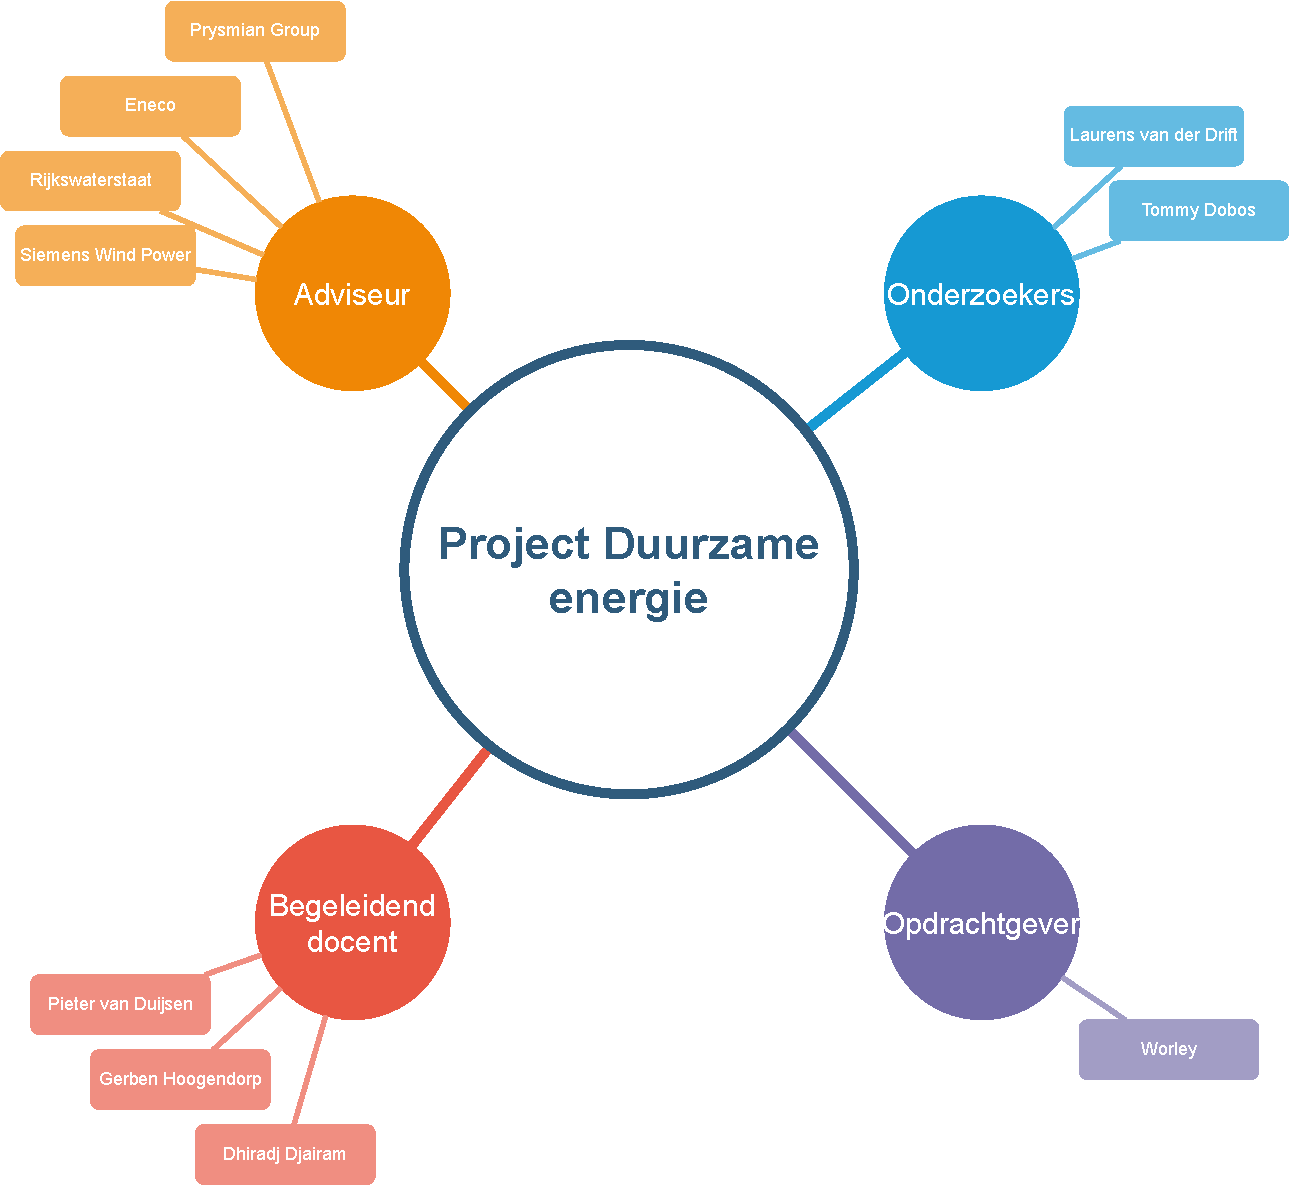
\includepdf[scale=0.65, pages=-]{mindmap/projectorganisatie.pdf}
\end{minipage}
% Onpersoonlijk:
\section{Planning} \label{planning}
De planning wordt beheerd via GitHub en omvat drie verschillende weergaven: Overview, ToDoList en roadmap.

In de \textbf{Overview}\textit{(zie figuur \ref{fig:overview})} wordt een samenvatting van alle taken getoond, inclusief de voltooide en de nog uit te voeren taken. Deze samenvatting omvat de volgende informatie:

    \textit{Repository}: Het project waaraan de taak is gekoppeld.\\
    \textit{Titel}: De naam van de opdracht.\\
    \textit{Assignees}: Verantwoordelijke personen voor de uitvoering van de opdracht.\\
    \textit{Status}: De voortgang van de opdracht.\\
    \textit{Startdatum en Deadline}: De begin- en einddatum van de opdracht.\\
    \textit{Prioriteit}: De urgentie van de opdracht.\\

\begin{figure}[h]
\centering
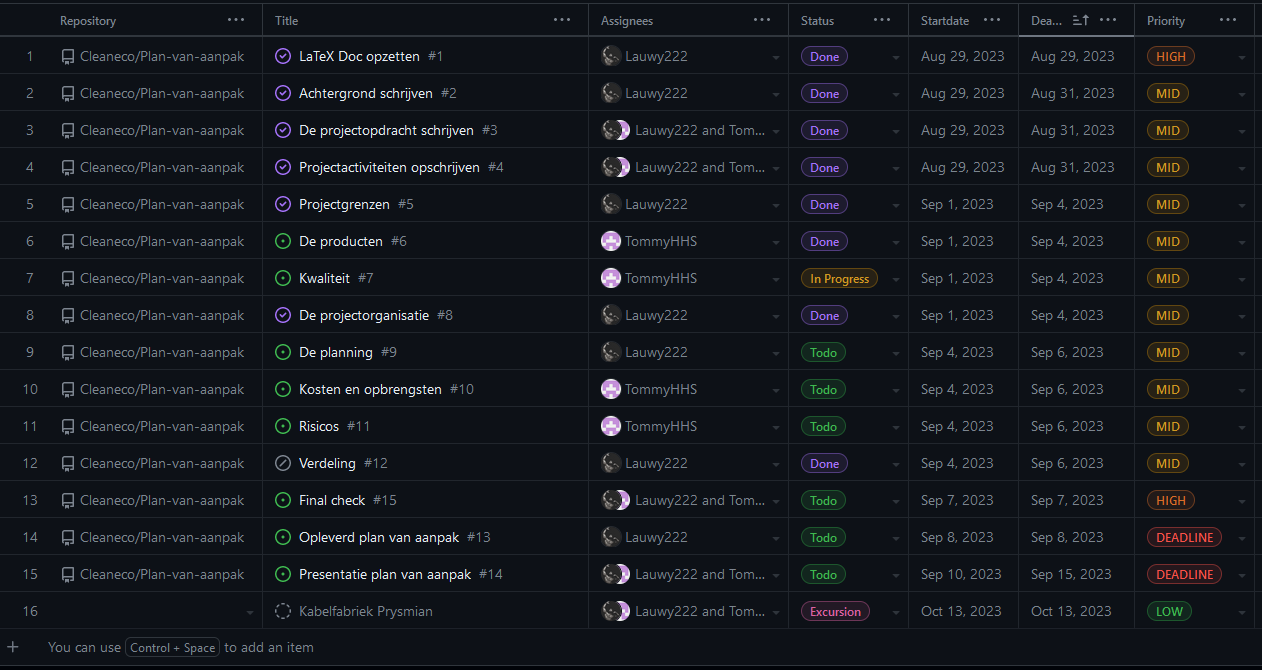
\includegraphics[width=0.9\textwidth]{IMG/overview.PNG}
\caption{Screenshot van de Overview in GitHub.}
\label{fig:overview}
\end{figure}

\newpage

In de \textbf{ToDoList}\textit{(zie figuur \ref{fig:todolist})} worden vier lijsten weergegeven en onderverdeeld onder vier categorieën: Te doen, In uitvoering, Voltooid en Excursie. Hier wordt aangegeven in welke fase van voltooiing elke opdracht zich bevindt, of deze nog moet worden uitgevoerd, in uitvoering is, is voltooid of betrekking heeft op een excursie die moet worden voorbereid.

\begin{figure}[h]
\centering
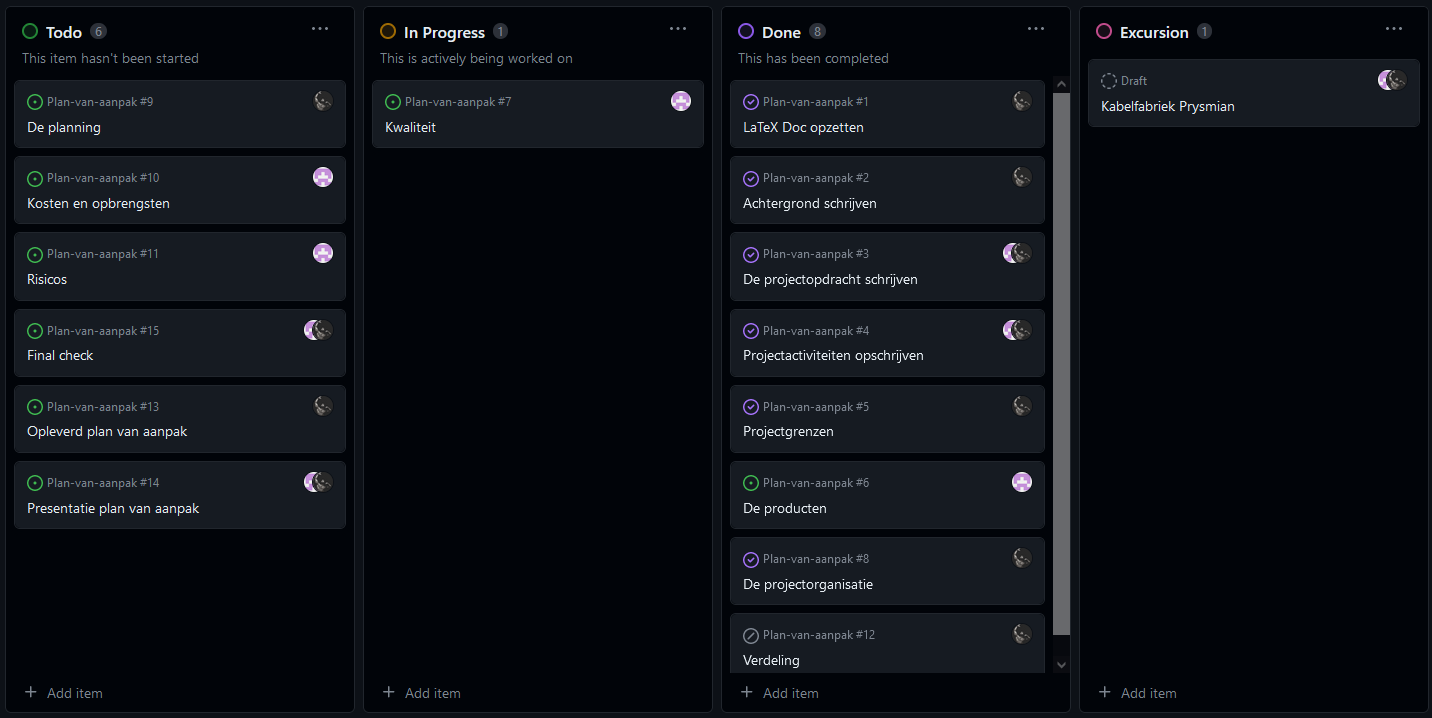
\includegraphics[width=0.9\textwidth]{IMG/todolist.PNG}
\caption{Screenshot van de ToDoList in GitHub.}
\label{fig:todolist}
\end{figure}

De \textbf{Roadmap}\textit{(zie figuur \ref{fig:roadmap})} biedt een visuele weergave van wanneer elke opdracht gepland was om te beginnen en wanneer de deadline is.

\begin{figure}[h]
\centering
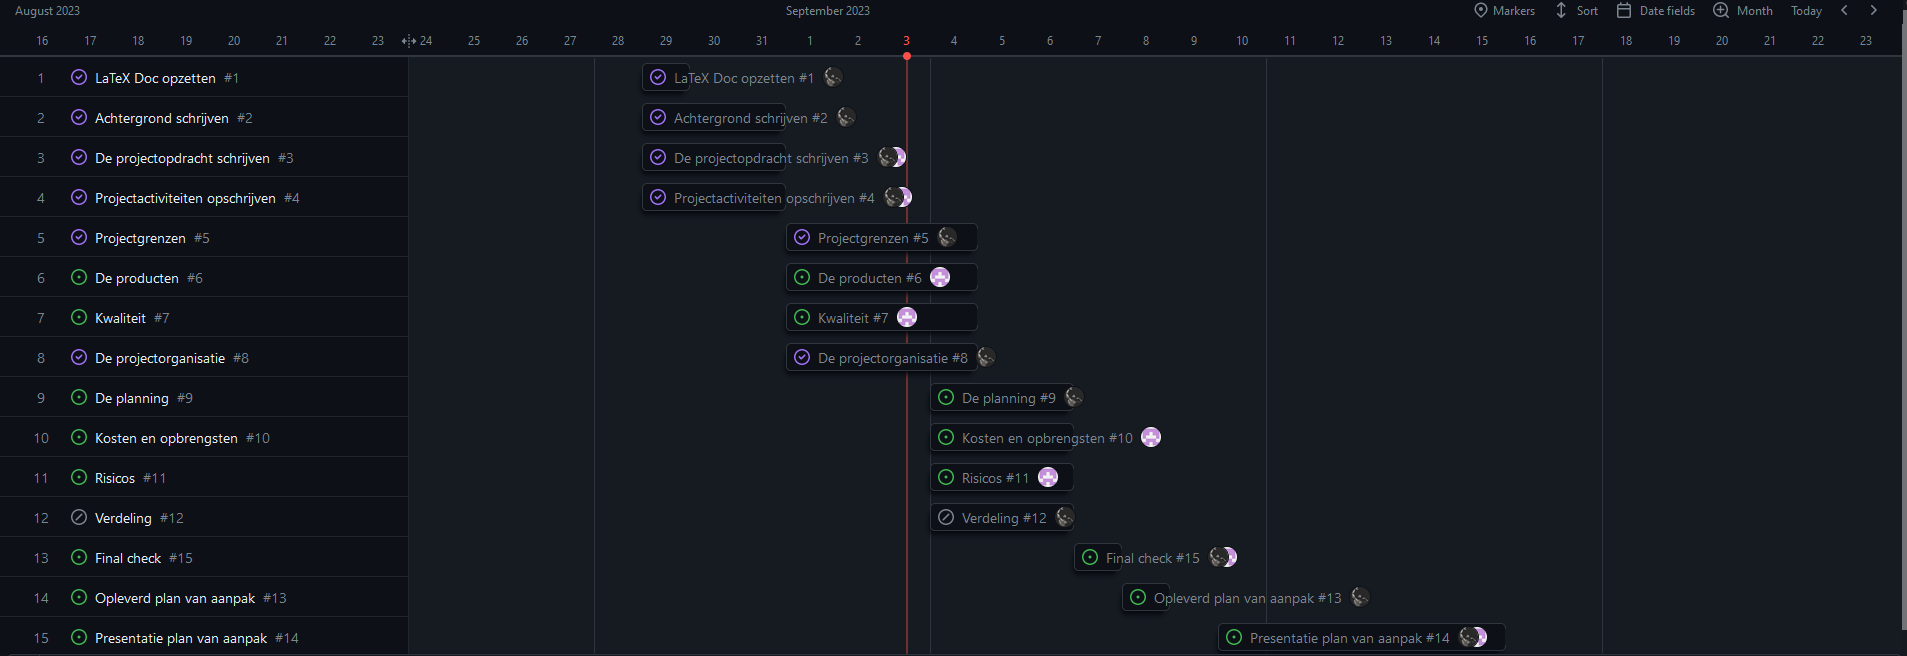
\includegraphics[width=0.9\textwidth]{IMG/roadmap.PNG}
\caption{Screenshot van de Roadmap in GitHub.}
\label{fig:roadmap}
\end{figure}

Indien er complicaties optreden tijdens het verloop van dit project, kunnen er tijdig opmerkingen worden geplaatst en om assistentie worden gevraagd. Hierdoor is er geen noodzaak voor fysieke vergaderingen en kan per opdracht aangegeven worden welke problemen zich voordoen en wat de projectstructuur nog verder verbetert.

% % SEMINEW
% \section{Planning} \label{planning}
% We gebruiken de Github planning met drie verschillende weergaven: Overview, ToDoList en roadmap.

% In het \textbf{Overview}\textit{(figuur:\ref{fig:overview})} tonen we een samenvatting van alle taken, inclusief degenen die zijn voltooid of nog moeten worden uitgevoerd, met devolgende informatie:

% - \textit{Repository}: Aan welk project het onderwerp is gekoppeld\\
% - \textit{Titel}: De naam van de opdracht\\
% - \textit{Assignees}: Wie verantwoordelijk is voor het uitvoeren van de opdracht\\
% - \textit{Status}: De voortgang van de opdracht\\
% - \textit{Startdatum} en Deadline: De begin- en einddatum van de opdracht\\
% - \textit{Prioriteit}: De urgentie van de opdracht\\

% \begin{figure}[h]
%     \centering
%     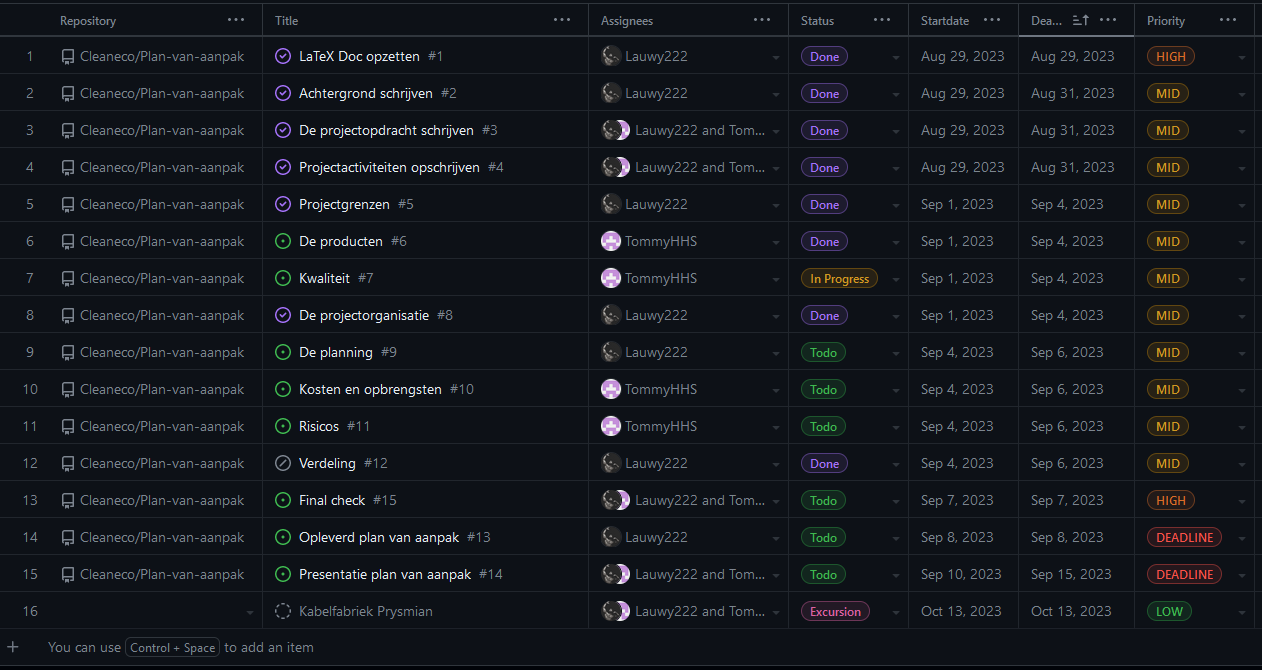
\includegraphics[width=0.9\textwidth]{IMG/overview.PNG}
%     \caption{Overview screenshot vanuit GitHub.}
%     \label{fig:overview}
% \end{figure}

% \newpage
% In de \textbf{ToDoList}\textit{(figuur:\ref{fig:todolist})} worden vier lijsten weergegeven en gecategoriseerd onder vier koppen: Te doen, In uitvoering, Voltooid en Excursie. Hier geven we aan in welke fase van voltooiing elke opdracht zich bevindt, of het nu nog moet worden gedaan, in uitvoering is, is voltooid, of het een excursie betreft die we moeten voorbereiden.

% \begin{figure}[h]
%     \centering
%     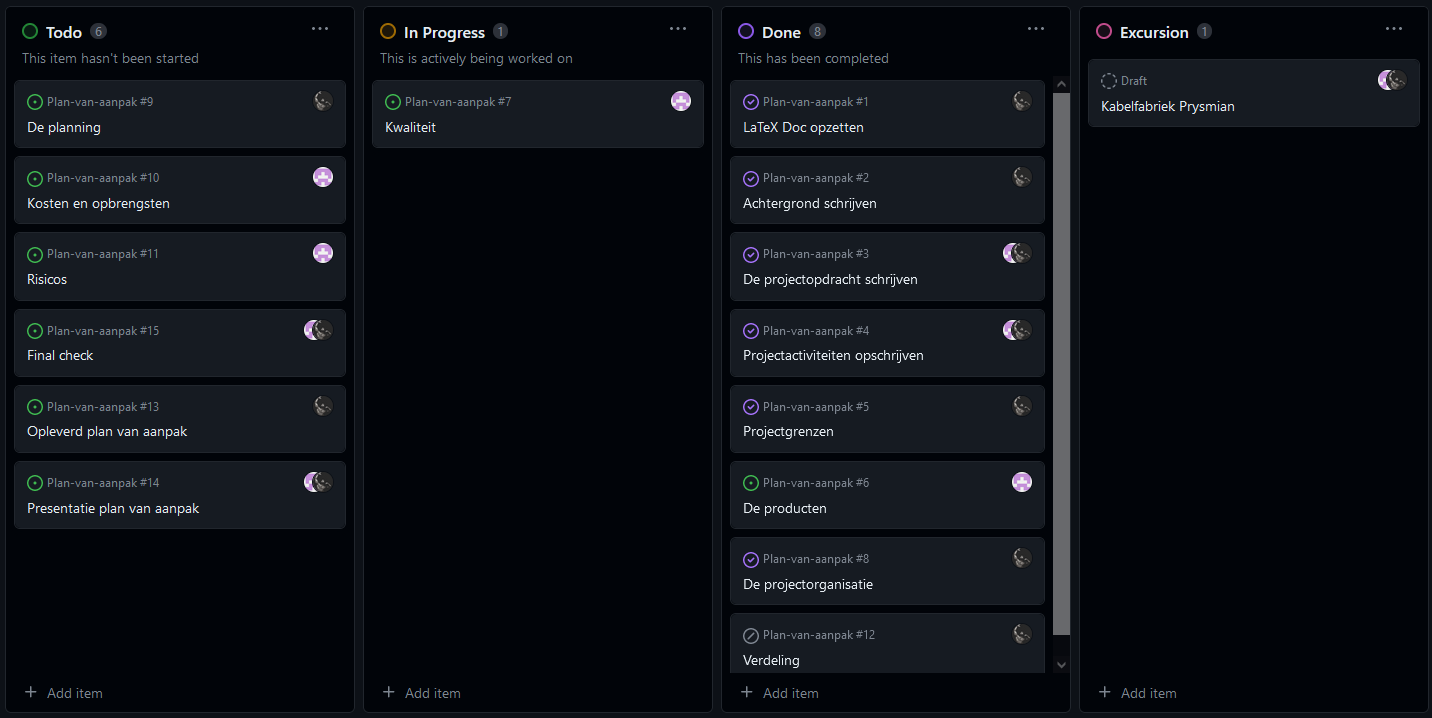
\includegraphics[width=0.9\textwidth]{IMG/todolist.PNG}
%     \caption{ToDoList screenshot vanuit GitHub.}
%     \label{fig:todolist}
% \end{figure}

% De \textbf{Roadmap}\textit{(figuur:\ref{fig:roadmap})} toont visueel wanneer een opdracht had moeten beginnen en wanneer de deadline is.

% \begin{figure}[h]
%     \centering
%     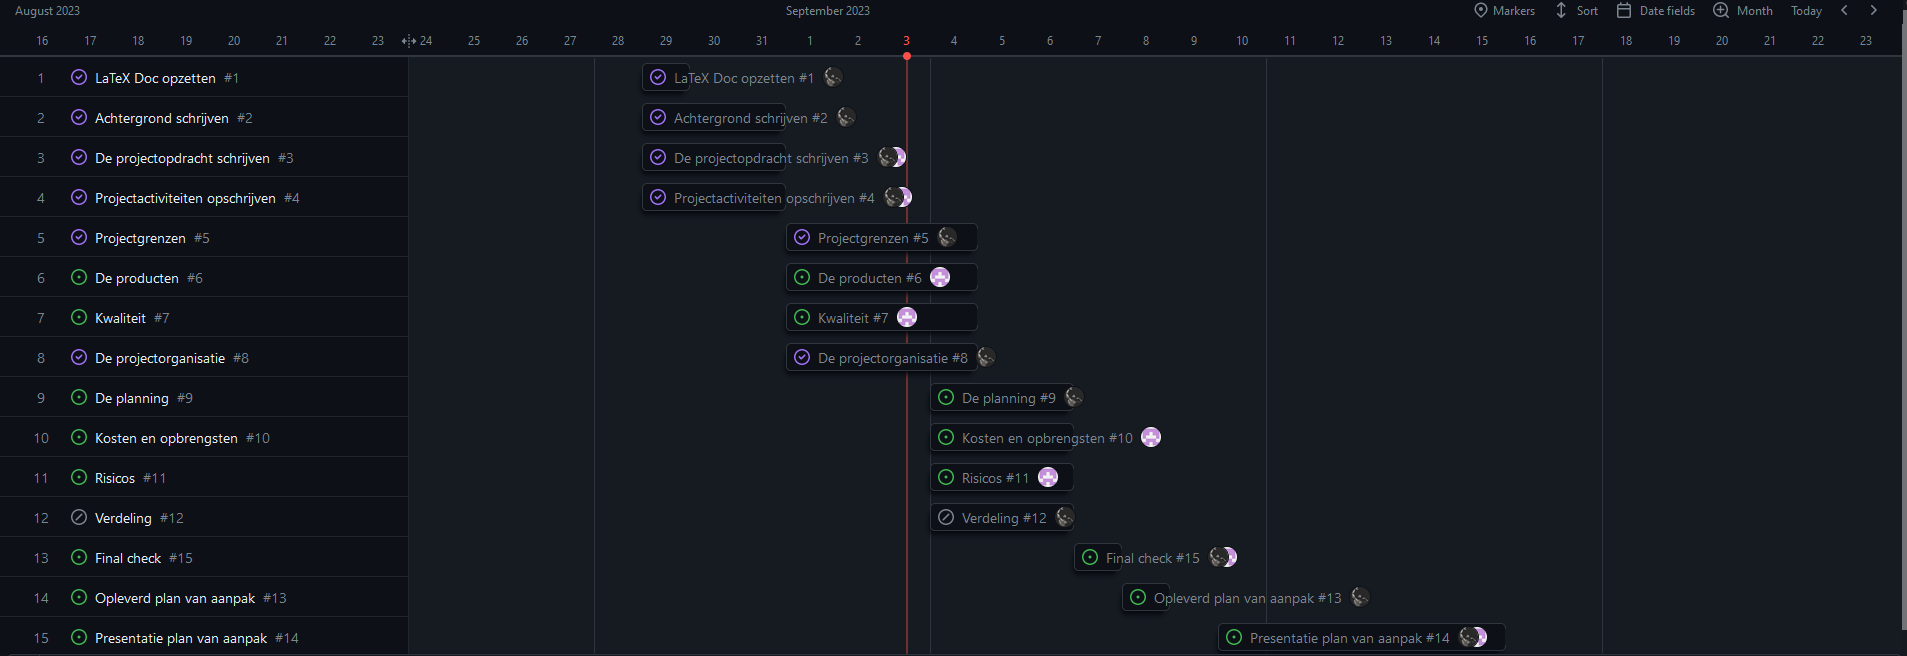
\includegraphics[width=0.9\textwidth]{IMG/roadmap.PNG}
%     \caption{Roadmap screenshot vanuit GitHub.}
%     \label{fig:roadmap}
% \end{figure}
% Als er complicaties optreden tijdens het proces van dit project, kunnen we op tijd een opmerking plaatsen en om hulp vragen. Op deze manier zijn we niet beperkt tot fysieke vergaderingen. We kunnen ook per opdracht aangeven wat niet lukt, waardoor alles nog gestructureerder verloopt.

% OLD

% \section{Planning} \label{planning}
% Wij hebben een planning in Github. Hierin geven wij het volgende aan:

% \textit{- Repository: Aan welk project het onderwerp is gekoppeld}

% \textit{- Title: wat is de titel van de opdracht}

% \textit{- Assignees: wie moet(en) de opdracht maken}

% \textit{- Status: hoe staat het ervoor met de opdracht}

% \textit{- Start-Date en Deadline: wat is de start- en einddatum van de opdracht}

% \textit{- Priority: wat is de urgentie van de opdracht}

% Wij hebben drie verschillende views: Overview, TodoList, Roadmap.

% Bij \textbf{Overview} wordt er een overzicht van alle taken laten zien die al gedaan zijn of nog moeten worden gedaan met extra informatie hierboven genoemd

% Bij \textbf{TodoList} worden er vier lijsten gevisualiseerd geindexeerd door vier kopjes. ToDo, In Progress, Done en Excursion. Hier geven we aan welke opdracht in welke status fase is of dat het een excursie is die wij moeten voorbereiden.

% Bij \textbf{Roadmap} wordt er gevisualiseerd wanneer een opdracht gestart moest zijn en wanneer de deadline is. 


% Mochten er complicaties voorkomen tijdens het process van dit project dan kunnen we optijd een comment plaatsen en vragen om hulp. Zo zijn wij dus niet gelimiteerd aan fysieke meetings. Ook kunnen wij per opdracht aangeven wat er niet lukt en alles dus nog gestructureerder is.


% Elke week worden er opdrachten gemaakt. Bij elke opdracht wordt een begin- en eindtijd gegeven. Het is de bedoeling dat de opdracht binnen deze tijd af is. Zodra dit niet het geval is, zal er eerst in overleg met de groepsleden besproken worden of de eindtijd verschoven mag/kan worden. Als daarentegen de ingeplande tijd voor de betreffende opdracht realistisch was en de opdracht niet af is, zal er in overleg met de opdrachtgever een kort gesprek moeten worden gevoerd om dit in de toekomst te voorkomen. Als er geen verbeteringen te zien zijn in de nabije toekomst, moeten er consequenties worden genomen door de groepsleden en de opdrachtgever.
% Voor de planning wordt Github gebruikt als tool om de opdrachten voor het project duidelijk weer te geven. In figuur 1 is te zien dat één opdracht uit zes kolommen bestaan. Daarin staat de:


% 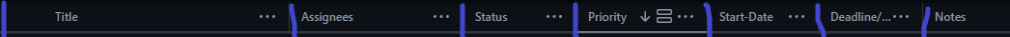
\includegraphics[width=6.7in]{IMG/08_planning_01.png} \\
% - Notes: wat moet er worden gedaan om de opdracht te voltooien
% In de opeenvolgende rijen daaronder worden alle opdrachten gemaakt met daarin de bijhorende informatie die in de bovenste kolommen gedefinieerd staan.
% \\\\
\section{Kosten en Opbrengsten}
    \subsection{Financiële kosten en budget}
    Bouwkosten Windpark: Hoewel specifieke bouwkosten niet worden vermeld in de verstrekte informatie, kan worden aangenomen dat de bouw van een windpark van 756 MW met 54 windturbines aanzienlijke kapitaalinvesteringen met zich meebrengt. Dit omvat de kosten voor het ontwerpen, fabriceren en installeren van de windturbines en de benodigde infrastructuur op zee.

    Milieueffectrapportages en Locatiestudies: Er wordt vermeld dat Ecowende kosten draagt voor milieueffectrapportages en locatiestudies. Deze studies zijn nodig om de impact van het windpark op het milieu en de omgeving te beoordelen en te minimaliseren.

    Overheidsinkomsten: De overheid ontvangt € 63,5 miljoen van de partijen als gevolg van financiële biedingen en bijdragen van Ecowende. Dit geld wordt gebruikt om nieuwe windparken beter te integreren in de omgeving en voor overige activiteiten op de Noordzee.

    \subsection{Tijdgebonden kosten}
Tijdslijn van het Project:

    2022: Ecowende, een \gls{joint venture} van Shell en Eneco, wint de vergunning voor het windpark Hollandse Kust (west) kavel VI.

    2023: Ontwerp en plannen worden gemaakt, en de bouw van het windpark is gepland om te beginnen in dit jaar.

    2026: Het windpark wordt naar verwachting volledig operationeel en levert elektriciteit.

Het maken van het windturbineparkontwerp en het onderhoudsplan zal gebeuren in een periode van 17 weken. Hiervan zal aan het begin ongeveer 60\% van de tijd besteed worden aan het maken van het windparkontwerp, de overige tijd zal worden gestoken in het realiseren van het onderhoudsplan en het verwerken van beide producten in het adviesrapport.\cite{studiewijzer} 

\subsection{Opbrengsten}

    Duurzame Energievoorziening: Het windpark Hollandse Kust (west) zal naar verwachting een vermogen van 756 MW genereren. Dit komt overeen met ongeveer 3\% van de Nederlandse elektriciteitsvraag, wat voldoende is om ongeveer een miljoen huishoudens van elektriciteit te voorzien. De opbrengst voor eindgebruikers is een toename van duurzame energievoorziening en een verminderde afhankelijkheid van niet-hernieuwbare bronnen zoals fossiele brandstoffen.

    Milieubescherming: Het ontwerp van het windpark is '\gls{natuurinclusief}' en omvat maatregelen om de impact op de natuur en het milieu te minimaliseren. Dit omvat bijvoorbeeld het creëren van een gezond ecosysteem, het minimaliseren van de impact op vogels, het onderwaterleven, en het stimuleren van biodiversiteit onder water. De opbrengst hier is een stap in de richting van milieubescherming en behoud van biodiversiteit.

    Toekomstige Groene Energie: Het windpark maakt deel uit van de groeiende inspanningen om groene energie in Nederland te vergroten. Dit draagt bij aan de ambitie om tegen 2030 ongeveer 21 GW aan windenergie op zee te hebben, wat een duurzame energiebron voor de toekomst zal opleveren.

    Economische Impuls: De bouw van windparken op zee kan een economische impuls geven aan de regio, met potentiële werkgelegenheidskansen in havens zoals Vlissingen, IJmuiden, Den Helder en de Eemshaven.

Samengevat, het project levert duurzame energie, milieubescherming, toekomstige groene energiebronnen en economische kansen op voor de eindgebruikers en de samenleving als geheel.\cite{Windenergiegebied}\cite{ShellEneco}\cite{Windopzee}

% Opbrengst:

% https://www.noordzeeloket.nl/functies-gebruik/windenergie/doorvaart-medegebruik/hollandse-kust-west/

% https://www.rvo.nl/onderwerpen/bureau-energieprojecten/afgesloten-projecten/woz-hollandse-kust-west-kavels-vi-vii

% https://www.rijksoverheid.nl/actueel/nieuws/2022/12/15/shell-en-eneco-winnen-tender-windpark-op-zee-hollandse-kust-west
\section{Risico’s}
Het ontwerpen van een windturbinepark en het opstellen van een onderhoudsplan zijn complexe projecten waarbij verschillende interne en externe risico's kunnen optreden. De risico´s kunnen verschillen van tijdsgebonden problemen tot technische complicaties. 

Het niet volledig begrijpen van de doelstellingen en eisen van het project, en/of onvoldoende communicatie tussen teamleden, belanghebbenden en experts kan resulteren in misverstanden, vertragingen, onsamenhangende of niet relevante informatie en overige fouten in de documenten. Daarom is, om dit te voorkomen, vooraf het plan van aanpak opgesteld. Daarnaast zal aan het begin van het project een analysefase plaatsvinden waarin de doelstellingen duidelijk worden voor de projectleden. Verder wordt er iedere week gecommuniceerd tussen de projectleden en worden wijzigingen in Github genoteerd. Zo wordt ervoor gezorgd dat op dit front niks fout gaat. 

Gebrek aan kennis kan ook zorgen voor problemen. Het projectteam heeft mogelijk onvoldoende kennis of ervaring met windturbineparkontwerp en -onderhoud, wat kan leiden tot onjuiste aanbevelingen. Het is daarom van belang dat het projectteam genoeg onderzoek doet en hun kennis uitbreid gedurende het project. Als het niet lukt de benodigde informatie te vinden of kennis op te doen, zal er naar alternatieve externen moeten worden gezocht voor hulp. Dit zal ervoor zorgen dat gebrek aan kennis geen barricade zal vormen, de teamleden hun kennis uitbreiden en toepassen om zo toch correcte en goede kwaliteit producten te kunnen leveren. 

Tijdsgebrek is ook een risico. Tijdsdruk om het parkontwerp en onderhoudsplan binnen strakke deadlines op te stellen, kan leiden tot gehaaste beslissingen en onvolledigheid van de documenten. Door goed te plannen en voor te bereiden zal dit worden voorkomen. 

Technologische veranderingen kunnen goed zijn, echter kan het ook voor problemen zorgen. Snelle technologische vooruitgang kan van invloed zijn op de keuze van apparatuur en systemen in het ontwerp en het onderhoudsplan, wat herziening noodzakelijk kan maken. Dit is een risico dat niet voorkomen kan worden. Het effect kan echter wel beperkt worden door op een bepaald moment een definitief besluit te nemen over de apparatuur en systemen die gebruikt zullen worden. 

Ten slotte zijn er nog financiële risico's. Beperkt budget kan de mogelijkheden limiteren. Daarnaast kunnen verschillende onverwachte gebeurtenissen gedurende het project zorgen voor verhoogde kosten. Mocht dit voorkomen, dan zal de situatie met de opdrachtgever besproken worden en zal gezocht worden naar een oplossing.
% \section{Verdeling van hoofdstukken}
 % Please add the following required packages to your document preamble:
% \usepackage[table,xcdraw]{xcolor}
% If you use beamer only pass "xcolor=table" option, i.e. \documentclass[xcolor=table]{beamer}
\begin{table}[h]
\begin{tabular}{|r|l|}
\hline
\rowcolor[HTML]{9B9B9B} 
\multicolumn{1}{|c|}{\cellcolor[HTML]{9B9B9B}\textit{\textbf{Hoofdstuk}}} & \multicolumn{1}{c|}{\cellcolor[HTML]{9B9B9B}\textit{\textbf{Teamlid}}} \\ \hline
\rowcolor[HTML]{EFEFEF} 
1 & Francisco Ramirez Ramirez \\ \hline
2 & Laurens van der Drift \\ \hline
\rowcolor[HTML]{EFEFEF} 
3 & Tommy Dobos \\ \hline
4 & Justin van der Reijden \\ \hline
\rowcolor[HTML]{EFEFEF} 
5 & Laurens van der Drift \\ \hline
6 & Tommy Dobos \\ \hline
\rowcolor[HTML]{EFEFEF} 
7 & Francisco Ramirez Ramirez \\ \hline
8 & Justin van der Reijden \\ \hline
\rowcolor[HTML]{EFEFEF} 
9 & Francisco Ramirez Ramirez \\ \hline
10 & Justin van der Reijden \\ \hline
\rowcolor [HTML]{EFEFEF}
Eindredactie & Tommy Dobos \\ \hline
\end{tabular}
\end{table}
\phantomsection
\addcontentsline{toc}{section}{Referenties}
\printbibliography
\end{document}
